% !TEX root = ../main.tex
\section{Dữ liệu}

\subsection{Dữ liệu phát hiện biển số}
Dữ liệu ảnh lấy từ bộ \emph{vietnamese-license-plate} (phiên bản 1) trên Roboflow Universe, workspace \code{school-fuhih}. Nhãn ở định dạng YOLO với một lớp duy nhất là \code{plate}. Ba tập con có sẵn của Roboflow được gộp lại rồi chia lại theo tỉ lệ 70/15/15 với hạt giống ngẫu nhiên cố định (seed 42). Ảnh tự thu thập (tiền tố \code{own\_}) luôn được đưa vào tập test, để tập test phản ánh điều kiện mà mô hình chưa từng thấy.

\begin{table}[H]
\centering
\caption{Phân chia dữ liệu phát hiện.}
\label{tab:split}
\begin{tabular}{lrr}
\toprule
Tập & Số ảnh & Số biển \\
\midrule
Train & 5\,849 & \todo{?} \\
Validation & 1\,254 & 1\,288 \\
Test & \todo{?} & \todo{?} \\
\bottomrule
\end{tabular}
\end{table}

\subsection{Dữ liệu nhận dạng chữ tổng hợp}
Bộ dữ liệu Roboflow chỉ có khung biển số, không có chuỗi ký tự. Để có dữ liệu huấn luyện CRNN, dự án xây dựng bộ sinh biển số tổng hợp (\code{src/alpr/synth.py}) gồm các bước:
\begin{enumerate}[nosep]
  \item \textbf{Sinh nội dung} ngẫu nhiên theo đúng định dạng Việt Nam: mã tỉnh 11--99, 50\,\% biển 2 dòng, phần số 5 chữ số với xác suất 0,8.
  \item \textbf{Vẽ biển} nền sáng, chữ tối, có viền, bằng font Hershey của OpenCV.
  \item \textbf{Tăng cường} để mô phỏng ảnh chụp thật: méo phối cảnh, xoay $\pm 5^\circ$, đổi độ sáng và tương phản, làm mờ do lệch nét hoặc do chuyển động, nhiễu cảm biến, giảm độ phân giải.
  \item \textbf{Tách dòng} biển 2 dòng bằng chính thuật toán dùng lúc suy luận (Mục~\ref{sec:split}).
\end{enumerate}
Tập huấn luyện gồm 50\,000 biển (khoảng 75\,000 ảnh dòng chữ). Tập kiểm định gồm 2\,000 biển sinh với hạt giống khác. Hình~\ref{fig:synth} minh hoạ một số mẫu.

\begin{figure}[H]
\centering
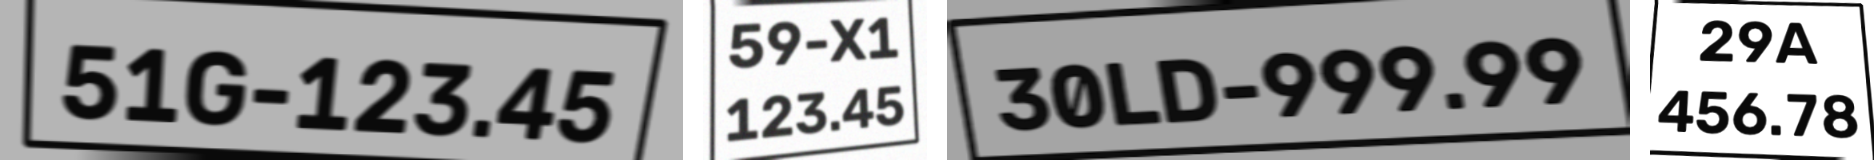
\includegraphics[width=\linewidth]{figures/synthetic.png}
\caption{Biển số tổng hợp sau khi tăng cường. Font Hershey khác font biển số thật, và đây là nguồn gốc của khoảng cách miền phân tích ở Mục~\ref{sec:error}.}
\label{fig:synth}
\end{figure}

\subsection{Định dạng nhãn chữ thật}
Để fine-tune CRNN và đánh giá end-to-end, dự án định nghĩa hai tệp nhãn:
\begin{itemize}[nosep]
  \item \code{texts.csv} (\code{image, plate\_idx, text}): chữ của từng khung biển, dùng để cắt ảnh dòng chữ huấn luyện. Hai dòng của biển 2 dòng phân cách bằng dấu \code{/}.
  \item \code{test\_texts.csv} (\code{image, text}): đáp án cho đánh giá end-to-end.
\end{itemize}
Tại thời điểm viết báo cáo, hai tệp này \textbf{chưa được gán nhãn}. Đây là hạn chế chính của kết quả thực nghiệm (Mục~\ref{sec:limit}).
